% Options for packages loaded elsewhere
\PassOptionsToPackage{unicode}{hyperref}
\PassOptionsToPackage{hyphens}{url}
\PassOptionsToPackage{dvipsnames,svgnames,x11names}{xcolor}
%
\documentclass[
  letterpaper,
  DIV=11,
  numbers=noendperiod]{scrreprt}

\usepackage{amsmath,amssymb}
\usepackage{lmodern}
\usepackage{iftex}
\ifPDFTeX
  \usepackage[T1]{fontenc}
  \usepackage[utf8]{inputenc}
  \usepackage{textcomp} % provide euro and other symbols
\else % if luatex or xetex
  \usepackage{unicode-math}
  \defaultfontfeatures{Scale=MatchLowercase}
  \defaultfontfeatures[\rmfamily]{Ligatures=TeX,Scale=1}
\fi
% Use upquote if available, for straight quotes in verbatim environments
\IfFileExists{upquote.sty}{\usepackage{upquote}}{}
\IfFileExists{microtype.sty}{% use microtype if available
  \usepackage[]{microtype}
  \UseMicrotypeSet[protrusion]{basicmath} % disable protrusion for tt fonts
}{}
\makeatletter
\@ifundefined{KOMAClassName}{% if non-KOMA class
  \IfFileExists{parskip.sty}{%
    \usepackage{parskip}
  }{% else
    \setlength{\parindent}{0pt}
    \setlength{\parskip}{6pt plus 2pt minus 1pt}}
}{% if KOMA class
  \KOMAoptions{parskip=half}}
\makeatother
\usepackage{xcolor}
\setlength{\emergencystretch}{3em} % prevent overfull lines
\setcounter{secnumdepth}{5}
% Make \paragraph and \subparagraph free-standing
\ifx\paragraph\undefined\else
  \let\oldparagraph\paragraph
  \renewcommand{\paragraph}[1]{\oldparagraph{#1}\mbox{}}
\fi
\ifx\subparagraph\undefined\else
  \let\oldsubparagraph\subparagraph
  \renewcommand{\subparagraph}[1]{\oldsubparagraph{#1}\mbox{}}
\fi

\usepackage{color}
\usepackage{fancyvrb}
\newcommand{\VerbBar}{|}
\newcommand{\VERB}{\Verb[commandchars=\\\{\}]}
\DefineVerbatimEnvironment{Highlighting}{Verbatim}{commandchars=\\\{\}}
% Add ',fontsize=\small' for more characters per line
\usepackage{framed}
\definecolor{shadecolor}{RGB}{241,243,245}
\newenvironment{Shaded}{\begin{snugshade}}{\end{snugshade}}
\newcommand{\AlertTok}[1]{\textcolor[rgb]{0.68,0.00,0.00}{#1}}
\newcommand{\AnnotationTok}[1]{\textcolor[rgb]{0.37,0.37,0.37}{#1}}
\newcommand{\AttributeTok}[1]{\textcolor[rgb]{0.40,0.45,0.13}{#1}}
\newcommand{\BaseNTok}[1]{\textcolor[rgb]{0.68,0.00,0.00}{#1}}
\newcommand{\BuiltInTok}[1]{\textcolor[rgb]{0.00,0.23,0.31}{#1}}
\newcommand{\CharTok}[1]{\textcolor[rgb]{0.13,0.47,0.30}{#1}}
\newcommand{\CommentTok}[1]{\textcolor[rgb]{0.37,0.37,0.37}{#1}}
\newcommand{\CommentVarTok}[1]{\textcolor[rgb]{0.37,0.37,0.37}{\textit{#1}}}
\newcommand{\ConstantTok}[1]{\textcolor[rgb]{0.56,0.35,0.01}{#1}}
\newcommand{\ControlFlowTok}[1]{\textcolor[rgb]{0.00,0.23,0.31}{#1}}
\newcommand{\DataTypeTok}[1]{\textcolor[rgb]{0.68,0.00,0.00}{#1}}
\newcommand{\DecValTok}[1]{\textcolor[rgb]{0.68,0.00,0.00}{#1}}
\newcommand{\DocumentationTok}[1]{\textcolor[rgb]{0.37,0.37,0.37}{\textit{#1}}}
\newcommand{\ErrorTok}[1]{\textcolor[rgb]{0.68,0.00,0.00}{#1}}
\newcommand{\ExtensionTok}[1]{\textcolor[rgb]{0.00,0.23,0.31}{#1}}
\newcommand{\FloatTok}[1]{\textcolor[rgb]{0.68,0.00,0.00}{#1}}
\newcommand{\FunctionTok}[1]{\textcolor[rgb]{0.28,0.35,0.67}{#1}}
\newcommand{\ImportTok}[1]{\textcolor[rgb]{0.00,0.46,0.62}{#1}}
\newcommand{\InformationTok}[1]{\textcolor[rgb]{0.37,0.37,0.37}{#1}}
\newcommand{\KeywordTok}[1]{\textcolor[rgb]{0.00,0.23,0.31}{#1}}
\newcommand{\NormalTok}[1]{\textcolor[rgb]{0.00,0.23,0.31}{#1}}
\newcommand{\OperatorTok}[1]{\textcolor[rgb]{0.37,0.37,0.37}{#1}}
\newcommand{\OtherTok}[1]{\textcolor[rgb]{0.00,0.23,0.31}{#1}}
\newcommand{\PreprocessorTok}[1]{\textcolor[rgb]{0.68,0.00,0.00}{#1}}
\newcommand{\RegionMarkerTok}[1]{\textcolor[rgb]{0.00,0.23,0.31}{#1}}
\newcommand{\SpecialCharTok}[1]{\textcolor[rgb]{0.37,0.37,0.37}{#1}}
\newcommand{\SpecialStringTok}[1]{\textcolor[rgb]{0.13,0.47,0.30}{#1}}
\newcommand{\StringTok}[1]{\textcolor[rgb]{0.13,0.47,0.30}{#1}}
\newcommand{\VariableTok}[1]{\textcolor[rgb]{0.07,0.07,0.07}{#1}}
\newcommand{\VerbatimStringTok}[1]{\textcolor[rgb]{0.13,0.47,0.30}{#1}}
\newcommand{\WarningTok}[1]{\textcolor[rgb]{0.37,0.37,0.37}{\textit{#1}}}

\providecommand{\tightlist}{%
  \setlength{\itemsep}{0pt}\setlength{\parskip}{0pt}}\usepackage{longtable,booktabs,array}
\usepackage{calc} % for calculating minipage widths
% Correct order of tables after \paragraph or \subparagraph
\usepackage{etoolbox}
\makeatletter
\patchcmd\longtable{\par}{\if@noskipsec\mbox{}\fi\par}{}{}
\makeatother
% Allow footnotes in longtable head/foot
\IfFileExists{footnotehyper.sty}{\usepackage{footnotehyper}}{\usepackage{footnote}}
\makesavenoteenv{longtable}
\usepackage{graphicx}
\makeatletter
\def\maxwidth{\ifdim\Gin@nat@width>\linewidth\linewidth\else\Gin@nat@width\fi}
\def\maxheight{\ifdim\Gin@nat@height>\textheight\textheight\else\Gin@nat@height\fi}
\makeatother
% Scale images if necessary, so that they will not overflow the page
% margins by default, and it is still possible to overwrite the defaults
% using explicit options in \includegraphics[width, height, ...]{}
\setkeys{Gin}{width=\maxwidth,height=\maxheight,keepaspectratio}
% Set default figure placement to htbp
\makeatletter
\def\fps@figure{htbp}
\makeatother

\KOMAoption{captions}{tableheading}
\makeatletter
\@ifpackageloaded{tcolorbox}{}{\usepackage[many]{tcolorbox}}
\@ifpackageloaded{fontawesome5}{}{\usepackage{fontawesome5}}
\definecolor{quarto-callout-color}{HTML}{909090}
\definecolor{quarto-callout-note-color}{HTML}{0758E5}
\definecolor{quarto-callout-important-color}{HTML}{CC1914}
\definecolor{quarto-callout-warning-color}{HTML}{EB9113}
\definecolor{quarto-callout-tip-color}{HTML}{00A047}
\definecolor{quarto-callout-caution-color}{HTML}{FC5300}
\definecolor{quarto-callout-color-frame}{HTML}{acacac}
\definecolor{quarto-callout-note-color-frame}{HTML}{4582ec}
\definecolor{quarto-callout-important-color-frame}{HTML}{d9534f}
\definecolor{quarto-callout-warning-color-frame}{HTML}{f0ad4e}
\definecolor{quarto-callout-tip-color-frame}{HTML}{02b875}
\definecolor{quarto-callout-caution-color-frame}{HTML}{fd7e14}
\makeatother
\makeatletter
\makeatother
\makeatletter
\@ifpackageloaded{bookmark}{}{\usepackage{bookmark}}
\makeatother
\makeatletter
\@ifpackageloaded{caption}{}{\usepackage{caption}}
\AtBeginDocument{%
\ifdefined\contentsname
  \renewcommand*\contentsname{Table of contents}
\else
  \newcommand\contentsname{Table of contents}
\fi
\ifdefined\listfigurename
  \renewcommand*\listfigurename{List of Figures}
\else
  \newcommand\listfigurename{List of Figures}
\fi
\ifdefined\listtablename
  \renewcommand*\listtablename{List of Tables}
\else
  \newcommand\listtablename{List of Tables}
\fi
\ifdefined\figurename
  \renewcommand*\figurename{Figure}
\else
  \newcommand\figurename{Figure}
\fi
\ifdefined\tablename
  \renewcommand*\tablename{Table}
\else
  \newcommand\tablename{Table}
\fi
}
\@ifpackageloaded{float}{}{\usepackage{float}}
\floatstyle{ruled}
\@ifundefined{c@chapter}{\newfloat{codelisting}{h}{lop}}{\newfloat{codelisting}{h}{lop}[chapter]}
\floatname{codelisting}{Listing}
\newcommand*\listoflistings{\listof{codelisting}{List of Listings}}
\usepackage{amsthm}
\theoremstyle{definition}
\newtheorem{exercise}{Exercise}[chapter]
\theoremstyle{remark}
\renewcommand*{\proofname}{Proof}
\newtheorem*{remark}{Remark}
\newtheorem*{solution}{Solution}
\makeatother
\makeatletter
\@ifpackageloaded{caption}{}{\usepackage{caption}}
\@ifpackageloaded{subcaption}{}{\usepackage{subcaption}}
\makeatother
\makeatletter
\@ifpackageloaded{tcolorbox}{}{\usepackage[many]{tcolorbox}}
\makeatother
\makeatletter
\@ifundefined{shadecolor}{\definecolor{shadecolor}{rgb}{.97, .97, .97}}
\makeatother
\makeatletter
\makeatother
\ifLuaTeX
  \usepackage{selnolig}  % disable illegal ligatures
\fi
\IfFileExists{bookmark.sty}{\usepackage{bookmark}}{\usepackage{hyperref}}
\IfFileExists{xurl.sty}{\usepackage{xurl}}{} % add URL line breaks if available
\urlstyle{same} % disable monospaced font for URLs
\hypersetup{
  pdftitle={TV2 Dataverwerking en statistiek},
  pdfauthor={Team TV},
  colorlinks=true,
  linkcolor={blue},
  filecolor={Maroon},
  citecolor={Blue},
  urlcolor={Blue},
  pdfcreator={LaTeX via pandoc}}

\title{TV2 Dataverwerking en statistiek}
\author{Team TV}
\date{6-9-2023}

\begin{document}
\maketitle
\ifdefined\Shaded\renewenvironment{Shaded}{\begin{tcolorbox}[enhanced, borderline west={3pt}{0pt}{shadecolor}, interior hidden, breakable, sharp corners, frame hidden, boxrule=0pt]}{\end{tcolorbox}}\fi

\renewcommand*\contentsname{Table of contents}
{
\hypersetup{linkcolor=}
\setcounter{tocdepth}{2}
\tableofcontents
}
\bookmarksetup{startatroot}

\hypertarget{inleiding}{%
\chapter*{Inleiding}\label{inleiding}}
\addcontentsline{toc}{chapter}{Inleiding}

Dit schooljaar gaan we weer verder met dataverwerking. Afgelopen jaar
hebben jullie de basis geleerd van hypothesetoetsen. Je weet hoe je een
aantal van die toetsen moet uitvoeren en je weet hoe je de output
daarvan moet interpreteren. Denk je nu ``nou, ik snap er nog geen hout
van'': kijk dan de stof van vorig jaar nog eens door, lees uit het boek
het het hoofdstuk over hypothesetoetsen en maak een paar oefenopgaven.

En jullie gaan deze kennis en vaardigheid natuurlijk gelijk inzetten in
jullie semesterprojecten!

Succes,

Team TV

\bookmarksetup{startatroot}

\hypertarget{hypothesetoetsen}{%
\chapter{Hypothesetoetsen}\label{hypothesetoetsen}}

\leavevmode\vadjust pre{\hypertarget{exr-hypothesetoetsen}{}}%
\begin{exercise}[Hypothesetoetsen]\label{exr-hypothesetoetsen}

In een experiment zijn 10 planten die meststof A hebben gekregen
vergeleken met 10 planten die meststof B hebben gekregen. Op de
plantmassa-data is een t-toets losgelaten. Er wordt getest met een
\(alpha\) van 0,05:

\begin{Shaded}
\begin{Highlighting}[]
\FunctionTok{library}\NormalTok{(tidyverse)}

\FunctionTok{set.seed}\NormalTok{(}\DecValTok{5}\NormalTok{) }\CommentTok{\# zet random steekproef vast}

\CommentTok{\# create dataset}
\NormalTok{df }\OtherTok{\textless{}{-}} \FunctionTok{data.frame}\NormalTok{(}\AttributeTok{meststof =} \FunctionTok{rep}\NormalTok{(}\FunctionTok{c}\NormalTok{(}\StringTok{"A"}\NormalTok{, }\StringTok{"B"}\NormalTok{), }\AttributeTok{each =} \DecValTok{10}\NormalTok{),}
                 \AttributeTok{plantlengte =} \FunctionTok{rnorm}\NormalTok{(}\DecValTok{20}\NormalTok{, }\DecValTok{5}\NormalTok{) }\SpecialCharTok{{-}} \FunctionTok{rep}\NormalTok{(}\FunctionTok{c}\NormalTok{(}\DecValTok{0}\NormalTok{, }\DecValTok{2}\NormalTok{), }\AttributeTok{each =} \DecValTok{10}\NormalTok{))}
\CommentTok{\#figure}
\FunctionTok{theme\_set}\NormalTok{(}\FunctionTok{theme\_classic}\NormalTok{(}\AttributeTok{base\_size =} \DecValTok{16}\NormalTok{))}

\FunctionTok{ggplot}\NormalTok{(df,}\FunctionTok{aes}\NormalTok{(meststof, plantlengte)) }\SpecialCharTok{+}
  \FunctionTok{stat\_summary}\NormalTok{(}\AttributeTok{geom =} \StringTok{"bar"}\NormalTok{, }\AttributeTok{fill =} \StringTok{"lightgrey"}\NormalTok{, }\AttributeTok{color =} \StringTok{"black"}\NormalTok{) }\SpecialCharTok{+}
  \FunctionTok{geom\_point}\NormalTok{(}\AttributeTok{color =} \StringTok{"blue"}\NormalTok{, }\AttributeTok{size =} \DecValTok{2}\NormalTok{, }
             \AttributeTok{position =} \FunctionTok{position\_nudge}\NormalTok{(}\AttributeTok{x =} \SpecialCharTok{{-}}\DecValTok{1}\SpecialCharTok{/}\DecValTok{5}\NormalTok{)) }\SpecialCharTok{+}
  \FunctionTok{stat\_summary}\NormalTok{(}\AttributeTok{geom =} \StringTok{"errorbar"}\NormalTok{, }\AttributeTok{width =} \FloatTok{0.3}\NormalTok{,}
               \AttributeTok{position =} \FunctionTok{position\_nudge}\NormalTok{(}\AttributeTok{x =} \DecValTok{1}\SpecialCharTok{/}\DecValTok{5}\NormalTok{)) }\SpecialCharTok{+}
  \FunctionTok{ylab}\NormalTok{(}\StringTok{"plantlengte (cm)"}\NormalTok{)}
\end{Highlighting}
\end{Shaded}

\begin{figure}[H]

{\centering \includegraphics{./Week1_files/figure-pdf/unnamed-chunk-1-1.pdf}

}

\end{figure}

\begin{Shaded}
\begin{Highlighting}[]
\FunctionTok{t.test}\NormalTok{(df}\SpecialCharTok{$}\NormalTok{plantlengte }\SpecialCharTok{\textasciitilde{}}\NormalTok{ df}\SpecialCharTok{$}\NormalTok{meststof)}
\end{Highlighting}
\end{Shaded}

\begin{verbatim}

    Welch Two Sample t-test

data:  df$plantlengte by df$meststof
t = 5.7731, df = 17.961, p-value = 1.815e-05
alternative hypothesis: true difference in means between group A and group B is not equal to 0
95 percent confidence interval:
 1.528639 3.278186
sample estimates:
mean in group A mean in group B 
       4.921148        2.517736 
\end{verbatim}

\begin{itemize}
\tightlist
\item
  Omschrijf de H\textsubscript{0} en de H\textsubscript{1}
\item
  omschrijf in eigen woorden wat de p-waarde betekent
\item
  Er komt een p-waarde uit van 0,02. Wat is de conclusie?
\item
  Hoe groot is de kans op een type-I-fout?
\end{itemize}

\end{exercise}

\begin{tcolorbox}[enhanced jigsaw, colbacktitle=quarto-callout-color!10!white, colframe=quarto-callout-color-frame, leftrule=.75mm, title={Warning}, coltitle=black, toprule=.15mm, colback=white, breakable, opacityback=0, bottomrule=.15mm, arc=.35mm, opacitybacktitle=0.6, bottomtitle=1mm, toptitle=1mm, rightrule=.15mm, titlerule=0mm, left=2mm]
Heb je moeite met bovenstaande opdracht, lees dan eerst nog eens goed
hoofstuk 6 van het boek \emph{The Analysis of Biological Data}.
\end{tcolorbox}

\hypertarget{power}{%
\section{Power}\label{power}}

Bij hypothesetoetsen doe je een uitspraak op basis van
waarschijnlijkheid. Daarbij kan je ofwel de juiste conclusie trekken,
danwel de verkeerde \ldots{}

Als de nulhypothese waar is, en je tóch de H\textsubscript{0} verwerpt,
dan maak je een type-I-fout. Die fout heb je in de hand, want dat is de
drempelwaarde \(alpha\) die je meestal op 0,05 stelt.

Maar ten onrechte de H\textsubscript{0} NIET verwerpen heb je minder
controle over. Deze fout wordt de type-II-fout genoemd.

\leavevmode\vadjust pre{\hypertarget{exr-type2fout}{}}%
\begin{exercise}[type-II-fouten]\label{exr-type2fout}

\begin{itemize}
\tightlist
\item
  omschrijf in eigen woorden de type-II-fout
\item
  bedenk 3 manieren om de kans op type-II-fout te verkleinen voor het
  voorbeeld van de vorige opgave
\end{itemize}

\end{exercise}

\hypertarget{meerdere-factoren}{%
\section{Meerdere factoren}\label{meerdere-factoren}}

\begin{Shaded}
\begin{Highlighting}[]

\NormalTok{Benoem voor ieder van de volgende *Experimental Designs* het onderscheidende kenmerk, en benoem de voordelen van dit kenmerk}

\NormalTok{* Factorial Design}
\NormalTok{* Randomized block design}
\NormalTok{* Completely randomized design}
\end{Highlighting}
\end{Shaded}

\hypertarget{power-berekenen}{%
\subsection{Power berekenen}\label{power-berekenen}}

De power van een toets is de waarschijnlijkheid dat, als er een verschil
is, deze ook wordt aangetoond (dus een p-waarde onder de drempelwaarde
\alpha).

\begin{tcolorbox}[enhanced jigsaw, colbacktitle=quarto-callout-note-color!10!white, colframe=quarto-callout-note-color-frame, leftrule=.75mm, title=\textcolor{quarto-callout-note-color}{\faInfo}\hspace{0.5em}{Note}, coltitle=black, toprule=.15mm, colback=white, breakable, opacityback=0, bottomrule=.15mm, arc=.35mm, opacitybacktitle=0.6, bottomtitle=1mm, toptitle=1mm, rightrule=.15mm, titlerule=0mm, left=2mm]
Voor de wiskundigen onder jullie: de power is gelijk aan 1 - de kans op
een type-II-fout.
\end{tcolorbox}

De power is afhankelijk van de volgende parameters:

\begin{itemize}
\tightlist
\item
  Het verschil tussen de twee groepen (in de situatie van een
  onafhankelijke t-toets).
\item
  De hoeveelheid (random!) variatie, meestal uitgedrukt met de term
  standaarddeviatie.
\item
  De gebruikte \alpha.
\item
  De hoeveelheid herhalingen
\end{itemize}

Weet je alle parameters, op een na, dan kan je die andere parameter
uitrekenen met de functie \texttt{power.t.test()}.

Het voorbeeld van plantlengte en bemesting. Ik weet het verschil en de
standaarddeviatie (want ik zelf die dataset verzonnen), en ik stel
\alpha op 0,05. Dan kan ik uitrekenen wat de power is voor het
experiment met 10 herhalingen:

\begin{Shaded}
\begin{Highlighting}[]
\FunctionTok{power.t.test}\NormalTok{(}\AttributeTok{n =} \DecValTok{10}\NormalTok{, }\AttributeTok{delta =} \DecValTok{2}\NormalTok{, }\AttributeTok{sd =} \DecValTok{1}\NormalTok{, }\AttributeTok{sig.level =} \FloatTok{0.05}\NormalTok{, }\AttributeTok{type =} \StringTok{"two.sample"}\NormalTok{, }\AttributeTok{alternative =} \StringTok{"two.sided"}\NormalTok{)}
\end{Highlighting}
\end{Shaded}

\begin{verbatim}

     Two-sample t test power calculation 

              n = 10
          delta = 2
             sd = 1
      sig.level = 0.05
          power = 0.988179
    alternative = two.sided

NOTE: n is number in *each* group
\end{verbatim}

Het argument n staat voor het aantal herhalingen per groep, delta staat
voor het verschil in gemiddelde tussen de groepen (wellicht kan je het
symbool \delta nog uit de wiskunde) en sd staat voor standaarddeviatie.
De power is het enige argument dat niet is ingevuld in de code, en deze
wordt dan ook uitgerekend. In dit geval is de power 0,99. Dat is enorm
hoog, meestal zijn we al tevreden met een power van 0,8!

\leavevmode\vadjust pre{\hypertarget{exr-powerberekenen}{}}%
\begin{exercise}[Power berekenen]\label{exr-powerberekenen}

\begin{itemize}
\tightlist
\item
  Verander bovenstaande code op zo'n manier dat je erachter komt hoeveel
  herhalingen je moet hebben om een power van 0,8 te krijgen.
\item
  Idem voor het geval je eenzijdig gaat toetsen.
\end{itemize}

\end{exercise}

\begin{tcolorbox}[enhanced jigsaw, colbacktitle=quarto-callout-color!10!white, colframe=quarto-callout-color-frame, leftrule=.75mm, title={Warning}, coltitle=black, toprule=.15mm, colback=white, breakable, opacityback=0, bottomrule=.15mm, arc=.35mm, opacitybacktitle=0.6, bottomtitle=1mm, toptitle=1mm, rightrule=.15mm, titlerule=0mm, left=2mm]
Heb je geen idee meer wat een- of tweezijdig toetsen is, lees dan nóg
een keer goed hoofstuk 6 van het boek \emph{The Analysis of Biological
Data}, en dan met name 6.5: \emph{One-sided tests}.
\end{tcolorbox}

\hypertarget{power-testen-in-de-praktijk}{%
\section{Power testen in de
praktijk}\label{power-testen-in-de-praktijk}}

In de praktijk weet je, voordag je een experiment gaat uitvoeren, niet
wat precies de variatie en het verschil zal zijn. Die moet je gaan
schatten vanuit de voorgaand experiment of vanuit de literatuur over
soortgelijke experimenten.

Wanneer je een inschatting hebt van de standaarddeviatie en het minimale
verschil wat je wilt kunnen aantonen, dan kan je voor een gekozen aantal
herhalingen berekenen wat de power is. Andersom kan ook: je wilt een
minimale power hebben (meestal minstens 0,8), dan kan je berekenen
hoeveel herhalingen je daar minimaal voor nodig hebt.

Neem nu weer als voorbeeld het experiment van de plantlengte. Stel dat
we alleen deze dat hebben en voor vervolgonderzoek willen uitvogelen
hoeveel herhalingen we nodig hebben.

De eerste vraag die je jezelf (of je opdrachtgever) moet stellen is
welke minimale verschil nog interessant is in de praktijk. In dit geval
gaat het om plantengroei, en een verschil van 0,5 cm in dit plantstadium
is voor de opdrachtgever nog interessant. Dan hebben we een delta van
0,5 cm.

Uit de voorgaande proef kunnen de standaarddeviatie halen. Dat vereist
wel wat stappen, omdat je de standaarddeviatie wilt hebben ten opzichte
van de gemiddeldes van beide groepen.

Dat worden de \textbf{residuen} genoemd. Voordat de residuen gebruikt
kunnen worden voor schatting van standaarddeviatie moeten die nog
gecorrigeerd worden voor de t-verdeling.

Dat doe je op de volgende manier:

\begin{Shaded}
\begin{Highlighting}[]
\CommentTok{\# eerst via functie het statistisch model schatten}
\NormalTok{t }\OtherTok{\textless{}{-}} \FunctionTok{lm}\NormalTok{(df}\SpecialCharTok{$}\NormalTok{plantlengte }\SpecialCharTok{\textasciitilde{}}\NormalTok{ df}\SpecialCharTok{$}\NormalTok{meststof)}
\CommentTok{\# vervolgens de, voor t{-}verdeling gecorrigeerde, residuen berekenen}
\NormalTok{r }\OtherTok{\textless{}{-}} \FunctionTok{rstudent}\NormalTok{(t)}
\CommentTok{\# en als laatste stap de standaarddeviatie berekenen}
\FunctionTok{sd}\NormalTok{(r)}
\end{Highlighting}
\end{Shaded}

\begin{verbatim}
[1] 1.091176
\end{verbatim}

Die schatting zit mooi dicht bij de werkelijke waarde (sd = 1).

\leavevmode\vadjust pre{\hypertarget{exr-powerberekenen2}{}}%
\begin{exercise}[Power berekenen in de
praktijk]\label{exr-powerberekenen2}

Herintroductie van zalm kan bemoeilijkt worden door de aanwezigheid van
forel. In een onderzoek hebben ecologen in verschillende beken waar
forel wel of niet aanwezig was zalmen uitgezet en gekeken welke fractie
zalmen overleefd had. De data staat in hoofdstuk 12 van \textbf{the
Analysis of Biological Data}, tabel 12.4.

\begin{itemize}
\tightlist
\item
  neem de data over in Excel
\item
  Maak en script waarin je de Excel importeert
\item
  voer een onafhankelijke t-toets uit op het effect van aanwezigheid
  forel op fractie overleven zalm.
\item
  voer nu de stappen uit om uit te rekenen hoeveel herhalingen je nodig
  hebt om het gevonden verschil statistisch hard te maken (met een power
  van 0,8). Haal daarbij het gemiddelde verschil en de standaardeviatie
  uit de dataset.
\end{itemize}

\end{exercise}

\bookmarksetup{startatroot}

\hypertarget{posthoctoetsen}{%
\chapter{Posthoctoetsen}\label{posthoctoetsen}}

\hypertarget{leerdoelen-deze-week}{%
\section{Leerdoelen deze week}\label{leerdoelen-deze-week}}

Met een \textbf{One-way ANOVA} kan je, i.t.t. de onafhankelijke t-toets,
meer dan twee groepen met elkaar vergelijken. Je hebt dan één
verklarende variabele van nominaal of ordinaal niveau, verdeeld in drie
of meer groepen. Je kan dat testen of de groepen van elkaar verschillen.
Wil je weten welke groepen onderling van elkaar verschillen, dan doe je
dat met een \textbf{posthoctoets}.

\begin{tcolorbox}[enhanced jigsaw, colbacktitle=quarto-callout-color!10!white, colframe=quarto-callout-color-frame, leftrule=.75mm, title={Warning}, coltitle=black, toprule=.15mm, colback=white, breakable, opacityback=0, bottomrule=.15mm, arc=.35mm, opacitybacktitle=0.6, bottomtitle=1mm, toptitle=1mm, rightrule=.15mm, titlerule=0mm, left=2mm]
Je mag alleen een posthoctoets uitvoeren als uit de anova een
significant effect komt. Dus altijd eerst de anova uitvoeren!
\end{tcolorbox}

Met een posthoctoets kan je groepen onderling vergelijken. Je voert het
uit om te kijken welke groepen onderling significant van elkaar
verschillen. Waarom niet gewoon een aantal t-toetsen uitvoeren (je
vergelijkt immers telkens twee groepen onderling)? Twee redenen:

\begin{itemize}
\tightlist
\item
  Ten eerste omdat je op zoek gaat of en waar onderlinge verschillen
  zitten. En voor al die toetsen bij elkaar wil je de kans op een
  type-1-fout (ten onrechte H\textsubscript{0} verwerpen) op 0,05
  houden.
\item
  Ten tweede omdat je dezelfde data gebruikt om verschillende toetsen
  uit te voeren.
\end{itemize}

\hypertarget{soorten-posthoctoetsen}{%
\section{Soorten posthoctoetsen}\label{soorten-posthoctoetsen}}

In de loop van de afgelopen eeuw zijn er heel wat verschillende
posthoctoetsen ontwikkeld en is het moeilijk door de bomen het bos te
zien. We gebruiken een aantal simpele stelregels:

\begin{itemize}
\tightlist
\item
  Alle groepen onderling vergelijken:

  \begin{itemize}
  \tightlist
  \item
    Bij ongeveer gelijke groepsgroottes: \textbf{Tukey HSD}.
  \item
    Bij ongelijke groepsgrootte: \textbf{Bonferroni}.
  \end{itemize}
\item
  Alleen behandelingen ten opzichte van een controlegroep vergelijken:

  \begin{itemize}
  \tightlist
  \item
    De \textbf{Dunnet's} posthoctoets.
  \end{itemize}
\end{itemize}

Hoe voeren we die uit (als voorbeeld met de melkgiftdata, waarbij
\texttt{fit} het resultaat is van de functie \texttt{lm()})?

Er zijn binnen R veel manieren om posthoctoetsen uit te voeren. Wij
gebruiken binnen deze cursus de package \textbf{emmeans}, omdat we met
deze package alle mogelijke posthoctoetsen kunnen uitvoeren. Wel zo
gemakkelijk.

In dit hoofstuk gebruiken we het voorbeeld van een studie naar melkgift
in verschillende koeienrassen:

\includegraphics{./Week2_files/figure-pdf/unnamed-chunk-1-1.pdf}

Je vindt de dataset op Teams.

\leavevmode\vadjust pre{\hypertarget{exr-koeien}{}}%
\begin{exercise}[Oneway-ANOVA Koeiendataset]\label{exr-koeien}

\begin{itemize}
\tightlist
\item
  Test eerst met een oneway-ANOVA of de rassen van elkaar verschillen in
  gemiddelde melkgift.
\item
  Welke conclusie trek je uit de toets?
\item
  Welke posthoctoets past bij deze dataset?
\end{itemize}

\end{exercise}

\hypertarget{de-functie-emmeans}{%
\section{de functie emmeans}\label{de-functie-emmeans}}

de functie \texttt{emmeans()} zit in de \emph{package} \textbf{emmeans}.
Packages kan je installeren met de functie \texttt{install.packages},
waarbij je als argument de naamvan de package tussen ``\,'' moet zetten.

\leavevmode\vadjust pre{\hypertarget{exr-installemmeans}{}}%
\begin{exercise}[emmeans installeren]\label{exr-installemmeans}

\begin{itemize}
\tightlist
\item
  installeer de package emmeans
\end{itemize}

\end{exercise}

Met de functie \texttt{emmeans} kan je van alles berekenen. Om het nog
complexer te maken kan je met verschillende argumenten in de functie
\texttt{emmeans()} dezelfde posthoctoets uitvoeren. Dat is goed om te
beseffen als op internet op zoek gaat naar codes voor posthoctoets. Hier
houden we een stijl aan die je voor iedere posthoctoets kan uitvoeren,
uitgevoerd op bijna ieder statistisch model:

\texttt{emmeans(fit,\ specs\ =\ \textasciitilde{}\ pairwise\ \textasciitilde{}\ variabele)}

Hierbij moet je voor \textbf{fit} de uitkomst van het statistisch model
zetten, en voor \textbf{variable} de naam van je verklarende variabele
waar je een posthoctoets op los wil laten. Eventueel kan je daar ook
(voor een two-way-ANOVA) meerdere verklarende variabelen neerzetten, op
dezelfde manier als in de functie \texttt{lm}, dus met een \texttt{+} of
een \texttt{*} tussen de namen.

\hypertarget{tukey-hsd}{%
\subsection{Tukey HSD}\label{tukey-hsd}}

Het resultaat bestaat uit twee onderdelen:

\begin{itemize}
\tightlist
\item
  Het gemiddelde effect van iedere factor (officieel de \emph{estimated
  marginal means} genoemd, weet je gelijk waar de naam van de package
  vandaan komt). Van ieder effect is ook de standaardfout en het
  betrouwbaarheidsinterval gegeven.
\item
  Daaronder staan de \emph{contrasts}. Dat zijn de onderlinge
  vergelijken. Het verschil wordt gegeven en er wordt een t-toets
  uitgevoerd waarbij de overschrijdingskans gecorrigeerd is. Standaard
  wordt de TukeyHSD-correctie gebruikt.
\end{itemize}

Hier is de uitkomst van de posthoctoets voor de koeiendata:

\begin{verbatim}
$emmeans
 ras emmean     SE df lower.CL upper.CL
 HF    2.95 0.0459  9     2.85     3.06
 MRY   3.21 0.0513  9     3.09     3.33
 RHF   2.97 0.0592  9     2.83     3.10

Confidence level used: 0.95 

$contrasts
 contrast  estimate     SE df t.ratio p.value
 HF - MRY   -0.2580 0.0688  9  -3.748  0.0114
 HF - RHF   -0.0147 0.0749  9  -0.196  0.9791
 MRY - RHF   0.2433 0.0784  9   3.105  0.0307

P value adjustment: tukey method for comparing a family of 3 estimates 
\end{verbatim}

De bovenste en onderste vergelijking zijn significant (p\textless0.05).
Dus MRY verschilt significant van HF en RHF, maar HF en RHF verschillen
onderling niet significant van elkaar.

\leavevmode\vadjust pre{\hypertarget{exr-tukey}{}}%
\begin{exercise}[Tukey HSD posthoctoets uitvoeren]\label{exr-tukey}

\begin{itemize}
\tightlist
\item
  Schrijf de code in een script voor het uitvoeren van bovenstaande
  Tukey HSD posthoctoets
\end{itemize}

\end{exercise}

\hypertarget{bonferroni}{%
\subsection{Bonferroni}\label{bonferroni}}

Willen we nu een Bonferroni-posthoc uitvoeren, dan hoeven maar een
argument toe te voegen:

\begin{Shaded}
\begin{Highlighting}[]
\FunctionTok{emmeans}\NormalTok{(fit, }\AttributeTok{specs =}\NormalTok{ pairwise }\SpecialCharTok{\textasciitilde{}}\NormalTok{ variabele, }\AttributeTok{adjust =} \StringTok{"bonf"}\NormalTok{)}
\end{Highlighting}
\end{Shaded}

Deze test is iets conservatiever (voorzichtiger) dus de p-waardes zijn
een fractie hoger.

\leavevmode\vadjust pre{\hypertarget{exr-bonf}{}}%
\begin{exercise}[Bonferroni posthoctoets uitvoeren]\label{exr-bonf}

\begin{itemize}
\tightlist
\item
  Schrijf de code in een script voor het uitvoeren van de Bonferroni
  posthoctoets voor de koeiendataset
\end{itemize}

\end{exercise}

\hypertarget{dunnets}{%
\subsection{Dunnet's}\label{dunnets}}

Voor de Dunnet's Posthoctoets gebruiken we als \emph{specs} niet de
pairwise, maar trt.vs.ctrl (*treatment versus control):

\begin{Shaded}
\begin{Highlighting}[]
\FunctionTok{emmeans}\NormalTok{(fit, }\AttributeTok{specs =}\NormalTok{ trt.vs.ctrl }\SpecialCharTok{\textasciitilde{}}\NormalTok{ variabele)}
\end{Highlighting}
\end{Shaded}

De functie pakt automatisch de eerste factor (hier \textbf{HF}) als
controle.

Met het argument `ref`` kan je aangeven welke factor je als controle
wilt. In onderstaand geval willen we de tweede factor als controle:

\begin{Shaded}
\begin{Highlighting}[]
\FunctionTok{emmeans}\NormalTok{(fit, }\AttributeTok{specs =}\NormalTok{ trt.vs.ctrl }\SpecialCharTok{\textasciitilde{}}\NormalTok{ ras, }\AttributeTok{ref =} \DecValTok{2}\NormalTok{)}
\end{Highlighting}
\end{Shaded}

Er is nog een variant voor als je de laatste factor als controle wilt.
Dan moet je een k achter ctrl zetten:

\begin{Shaded}
\begin{Highlighting}[]
\FunctionTok{emmeans}\NormalTok{(fit, }\AttributeTok{specs =}\NormalTok{ trt.vs.ctrlk }\SpecialCharTok{\textasciitilde{}}\NormalTok{ ras)}
\end{Highlighting}
\end{Shaded}

\hypertarget{resultaten-posthoctoets-in-ggplot}{%
\section{Resultaten Posthoctoets in
ggplot}\label{resultaten-posthoctoets-in-ggplot}}

Het is gebruikelijk om in figuren met hoofdletters aan te geven welke
groepen van elkaar verschillen. Kijk maar eens in een wetenschappelijk
artikel waarin staafdiagrammen staan.

Als we terug gaan naar het voorbeeld van de koeien, dan hebben we de
volgende output uit de Tukey HSD posthoctoets:

\begin{verbatim}
$emmeans
 ras emmean     SE df lower.CL upper.CL
 HF    2.95 0.0459  9     2.85     3.06
 MRY   3.21 0.0513  9     3.09     3.33
 RHF   2.97 0.0592  9     2.83     3.10

Confidence level used: 0.95 

$contrasts
 contrast  estimate     SE df t.ratio p.value
 HF - MRY   -0.2580 0.0688  9  -3.748  0.0114
 HF - RHF   -0.0147 0.0749  9  -0.196  0.9791
 MRY - RHF   0.2433 0.0784  9   3.105  0.0307

P value adjustment: tukey method for comparing a family of 3 estimates 
\end{verbatim}

Je ziet dat de volgorde van effect HF \textgreater{} RHF \textgreater{}
MRY is. HF en RHF verschillen significant van MRY (p-waarde \textless{}
0,05), maar verschillen niet onderling (p-waarde = 0,9791). Normaal geef
je de laagste waarde een A en significant hogere waarden de volgende
letters in het alfabet. In dit geval krijgen:

\begin{Shaded}
\begin{Highlighting}[]
\FunctionTok{ggplot}\NormalTok{(koeien, }\FunctionTok{aes}\NormalTok{(ras, Melksnelheid)) }\SpecialCharTok{+}
  \FunctionTok{stat\_summary}\NormalTok{(}\AttributeTok{geom =} \StringTok{"bar"}\NormalTok{, }\AttributeTok{fill =} \StringTok{"lightblue"}\NormalTok{) }\SpecialCharTok{+}
  \FunctionTok{stat\_summary}\NormalTok{(}\AttributeTok{geom =} \StringTok{"errorbar"}\NormalTok{, }\AttributeTok{width =} \FloatTok{0.3}\NormalTok{) }\SpecialCharTok{+}
  \FunctionTok{stat\_summary}\NormalTok{(}\AttributeTok{geom =} \StringTok{"text"}\NormalTok{, }\AttributeTok{label =} \FunctionTok{c}\NormalTok{(}\StringTok{"A"}\NormalTok{, }\StringTok{"B"}\NormalTok{, }\StringTok{"A"}\NormalTok{), }\AttributeTok{vjust =} \SpecialCharTok{{-}}\FloatTok{0.6}\NormalTok{, }\AttributeTok{size  =} \DecValTok{8}\NormalTok{) }\SpecialCharTok{+}
  \FunctionTok{ylim}\NormalTok{(}\FunctionTok{c}\NormalTok{(}\DecValTok{0}\NormalTok{, }\DecValTok{4}\NormalTok{))}
\end{Highlighting}
\end{Shaded}

\begin{figure}[H]

{\centering 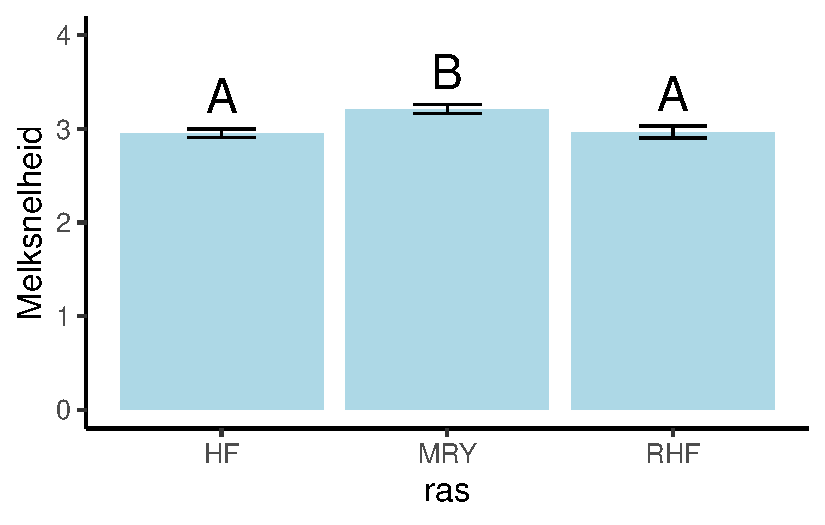
\includegraphics{./Week2_files/figure-pdf/unnamed-chunk-8-1.pdf}

}

\end{figure}

De functie \texttt{stat\_summary} kan je ook gebruiken om tekst toe te
voegen. Voordeel is dat die dezelfde datapunten meeneemt als de
voorgaande regels code (voor \emph{bar} en \emph{errorbar}). Hierdoor
komt de tekst op de goede plek. Je moet wel spelen met de code om de
figuur netjes te maken. Ten eerst wil je de letter boven de staven
hebben, dat doe je met het argument \texttt{vjust}. Negatieve waardes
betekent omhoog, positieve waardes omlaag. De beste waarde is natuurlijk
afhankelijk van hoe groot je foutenbalken zijn. Daarnaast wil je de
letters ook groot genoeg hebben (naar eigen smaak), met het argument
\texttt{size}. Maar hierdoor kunnen de letters voorbij de bovenkant
gaan. Dat los je weer op door de schaal op de y-as te veranderen met de
functie \texttt{ylim}.

\leavevmode\vadjust pre{\hypertarget{exr-CapLet}{}}%
\begin{exercise}[Spielerei met ggplot]\label{exr-CapLet}

\begin{itemize}
\tightlist
\item
  Neem bovenstaande code over en past die aan naar eigen smaak. NB:
  bovenstaande figuur heeft als \emph{theme} \textbf{theme\_classic}.
  Zelf zet ik dat thema al bovenaan mijn script vast (na
  \texttt{library(tidyverse})) met de functie
  \texttt{theme\_set(theme\_classic())}.
\end{itemize}

\end{exercise}

\hypertarget{opgaven-hoofdstuk-15}{%
\section{Opgaven hoofdstuk 15}\label{opgaven-hoofdstuk-15}}

\leavevmode\vadjust pre{\hypertarget{exr-postdocoefeningen}{}}%
\begin{exercise}[\textbf{Practice
Problems}]\label{exr-postdocoefeningen}

Gebruik uit onderstaande \emph{Practice Problems} de datasets:

15.1, 15.4, 15.8

I.p.v. vragen uit het boek, met dezelfde dataset de volgende vragen
beantwoorden:

\begin{itemize}
\tightlist
\item
  Data invoeren
\item
  Scatterplot maken
\item
  Hypotheses opstellen
\item
  ANOVA uitvoeren, p-waarden opschrijven
\item
  De juiste posthoc-toets uitvoeren
\item
  Conclusies trekken
\end{itemize}

\end{exercise}



\end{document}
